\documentclass[Main/main.tex]{subfiles}

\begin{document}

\section{Theory and Methods}
%SOPs!
%Reasonable level of detail
%Sufficient detail how you have planned and conducted your experimetal work
%Everything needed to understand discussions

%Experimental design, method for synthesis - equqtions and structures
%Instrumentation, analytic methods - SOP, numbers, type of instruments
%Samples, chemicals, materials
%Preparation and storage - commercial source 
%Models and statistical tools

\subsection{Electrochemistry}

\subsubsection{Electrochemical cells}

A battery consists of one or more interconnected electrochemical cells each supplying a current ($I$) at a voltage ($V$) for a time $\Delta t$. For a battery to be rechargeable, the chemical reaction occuring inside the cell needs to be reversible on the application of charging \textit{I} and \textit{V}.

The electrolyte separating the anode and the cathode may be liquid or solid. Solid electrolytes are often used with gaseous or liquid electrodes while a liquid electrolyte commonly is in use whith solid electrodes. In the latter, the electrodes are kept apart by an electrolyte-permeable separator. As can be seen from figure \ref{fig:2_jacs}, the electrolyte permits the ionic component of the redox reaction (occuring at the electrodes) through while forcing the electronic component to do work by traversing an external circuit. 

\begin{figure}[h]
	\centering
	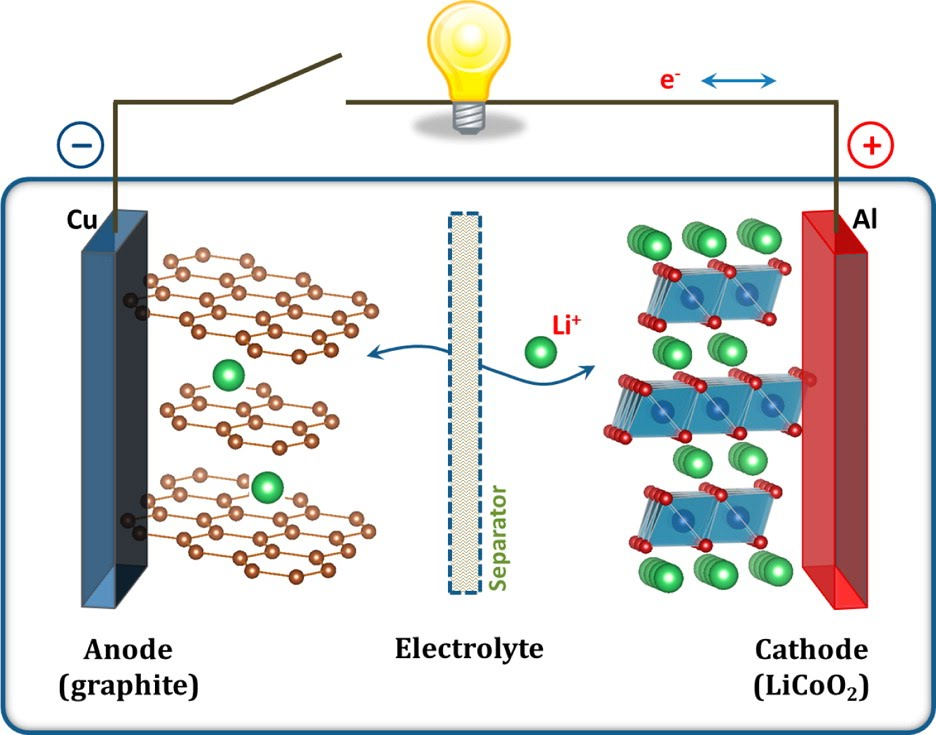
\includegraphics[width=0.7\linewidth]{uploads/JACS}
	\caption{Schematic of the firs Li-ion battery. Ions are permitted through the electrolyte while electrons traverse the external circuit.}
	\label{fig:2_jacs}
\end{figure}


$Q(I)$ is the cell capacity for a given current, $I$. $Q$ is the total charge per unit weight (\si{Ah\ kg^{-1}}/\si{mAh\ g^{-1}}) or per volume (\si{Ah\ L^{-1}}). The dependency of $I$ arises since the rate of transfer of ions becomes diffusion-limited at high currents. 

A perfect battery would be able to dispatch the same charge on discharge as it is supplied while charging - every time. In other words, there should ideally not be any capacity fade throughout the life of the battery. A diffusion-limited loss of ions presents a reversible loss of capacity. However, changes in electrode volume, electrode decomposition or chemical reactions between electrode and electrolyte may cause an irreversible loss of capacity \cite{2_Goodenough_perspective}.

The Coloumbic efficiency, \[ 100 \times \frac{Q_{dis}}{Q_{ch}} \] gives the efficiency of a single cycle associated with capacity fade. The cycle life of a battery is then the amount of cycles the battery can withstand before the capacity has faded to $80\%$ of its initial reversible value.


\textbf{Something about SEI?}
YES

\subsubsection{How batteries typically are made}

Binder and carbon additive 


\subsection{Scanning Electron Microscope (SEM)}
The scanning electron microscope scans a focused electron beam over the surface area of a specimen, examining(?) the microscopic structure with a higher resolution and much greater depth of field compared to an optical microscope. The large depth of field results in a three-dimensional appearance of its images. In addition, chemical information from a specimen can be obtained through the use of various techniques, including using a X-ray energy-dispersive spectrometer (EDS).

A SEM is composed of an electron gun and a series of electromagnetic lenses and apertures. 
*electron source
*Detectors (SE and BSE)

\subsection{X-ray diffraction (XRD)}
X-rays are a form of electromagnetic radiation with wavelengths ranging from 0.1 to 100 \si{\angstrom}, first discovered by Wilhelm C. Röntgen in 1895. These wavelengths are in the order of interatomic distances in crystals causing diffracted waves to form a unique diffraction pattern due to interference. Thus, X-rays has proven to be an excellent probe of the structure of matter \cite{2_XRD,Scotman}.

The condition for constructive interference is described by Bragg's law as
    $$n\lambda = 2d\sin{\theta}$$
where \textit{n} is an integer, \textit{d} is the lattice spacing, \textit{$\lambda$} is the wavelength of the diffracted beam and \textit{$\theta$} is the diffraction angle. An illustration of the geometry is shown in figure \ref{fig:bragg}.

\begin{figure}[ht]
    \centering
    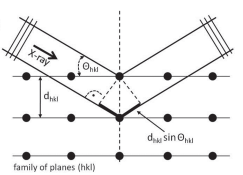
\includegraphics{uploads/Bragg.PNG}
    \caption{Visualization of the principles used to derive Bragg's law \cite{Scotman}}
    \label{fig:bragg}
\end{figure}

By plotting the counted reflections as a function of the angle between the incident and the diffracted beam (angle of diffraction), the positions and intensities of the peaks works as a fingerprint for the identification of unknown materials by comparing the diffraction pattern with a reference database. Further comprehensive analysis can supply information regarding bond lengths, bond angles, structural disorder and more. \cite{Scotman}.




\subsection{Electrochemical analysis}
When investigating the electrochemical properties of a battery, the cell voltage and the current are often the main parameters of interest. With one of these parameters fixed and the other monitored, valuable information regarding the electrochemical properties can be obtained. 

\subsubsection{Impedance}
Impedance is a measurement of the opposition a circuit presents to a current with an applied voltage. Impedance possesses both magnitude and phase and extends the concept of resistance to alternating current (AC) circuits. Thus, Ohm's law can be modified to $V = ZI$, where $Z$ is impedance and $Z=R$ for a pure resistor.

\subsubsection{Cyclic voltammetry}
Cycling voltammetry (CV) is a highly versatile and useful technique commonly employed to investigate the reduction and oxidation properties of a given material. In addition, CV is used to study electron transfer-initiated chemical reactions \cite{2_CV}. During CV, current is measured as a function of applied voltage. With a minimum and maximum voltage set, the measurement starts at zero current voltage (0CV). From there, the voltage is swept at at constant scan rate to the maximum voltage, then to the minimum voltage and ends up at 0CV. This scan is repeated for a number of cycles.

*Scan rate
CV 

\subsubsection{Galvanostatic cycling}
During galvanostatic cycling a constant current is pushed into or out of the battery



\subsection{Liquid injection system under vacuum}
The main goal of this thesis is to explore a novel system for the formation of oxides from a variety of more or less complex compounds. The system produces powder that sticks to the surfaces present during the synthesis. Liquid is injected in pre-determined amounts (droplets) into a round bottom flask under vacuum and heated. The liquid evaporates (do I know that it evaporates?) and decomposes into oxides which are then deposited on the substrates present in the flask as well as the surface of the flask itself.

This behaviour can be exploited to synthesize cathodes without the need for a binder in order to have the oxide stick to a conducting surface. 


\section{Experimental design}

This section will give an overview of the instrumentation used in this thesis. Since the deposition technique used is a new method, the level of detail will be more extensive.

\subsection{Liquid injection system}
The system consisted of a 500 ml single-neck round-bottom flask with a joint size of 29/32 (29 mm wide at the top and 32 mm long) attached to a connector pipe, sealed with a Teflon cone  and silicon grease. A 1/16” stainless steel tube, henceforth called injector-tube  , went from a 6-port Valco valve, through a cap on top of the connector tube and down to the bottom of the neck of the flask. A vacuum pump was connected to the connector tube in order to reduce the pressure of the flask and the pressure was monitored with the use of a Pirani gauge. A heating mantle and aluminum foil was used to heat the round-bottom flask to 300-400 $\degree C$ during the injection.

In addition to the injector-wire, the 6-ports valve connects a 10 m L syringe containing the precursor, a steel tube forming a loop, an open-end tube and a tube supplying nitrogen gas. The 6-ports valve was used in two different positions, controlled by an Arduino  . The first position allowed for the tube to be filled with the precursor. The precursor was mechanically injected from the syringe and any excess liquid went into a waste beaker from the open-end tube. The second position opened for a nitrogen flow to push the liquid from the tube through the injector-wire and into the round-bottom flask. A schematic of the apparatus is presented in figure \ref{fig:ehhh1}. 

Two different vacuum pumps were used due to malfunction of the first pump halfway through the experiments, first a rotary vane pump and secondly a membrane pump. *  

During the preparation for new runs, a round-bottom flask was washed and dried, 10 mL of the precursor solution measured in the syringe and all the substrates blown and washed with ethanol, before carefully placing them in the flask. A variety of glass, Si and steel plates were utilized. Between the runs, the round-bottom flasks were washed in an acid bath, removing most of the deposited material from the previous run. Any residual material that did not get washed away with either acid or water and a brush were considered to not affect the consecutive run.


\subsubsection{Parameter testing}
Since this is a novel system, various parameters has been altered in order to see their effect on the synthesized material. The main parameters of interest has been the position of the tip of the injector-wire and the concentration of the precursor(s). 

\subsubsection{Cathode production}

\begin{itemize}
    \item The whole shabang - Round-bottom flask, vacuum tube, connector pipe, silicon grease and cones(?), vacuum pump (two different, second somewhat lower pressure), alu foil, sample holder, glass substrates, Si substrates, metal plates (spacers), 6-ports valve, heating mantle \todo{Missing something?}
    \item Software used?
    \item Making batteries
    \item Compounds. Just state the stochiometry and such or show how I have derived it?
    \item Limitations from the equipment?
    \item How detailed about the runs? Placement of substrates in the flask? Dimensions of substrates and sample holder?
\end{itemize}

\begin{figure}[p]
\centering
\includegraphics[width=1\linewidth]{uploads/ehhh1}
\caption{Schematic of the liquid injection system}
\label{fig:ehhh1}
\end{figure}


\subsection{Chemicals used}

\begin{figure}[ht]
	\centering
	\resizebox{\textwidth}{!}{
		\begin{tabular}{cccccc}
			\hline 
			\textbf{Compound} & \textbf{Linear formula} & \textbf{Purity} & \textbf{Supplier} & \textbf{CAS} & \textbf{Lot \#} \\ 
			\hline 
			Manganese(II) nitrate hydrate & \ce{Mn(NO3)2.xH2O} & 98\% & Sigma-Aldrich & 15710-66-4 & MKBR0853V \\
			
			Lithium nitrate & \ce{LiNO3} & $>$ 99\% & Sigma-Aldrich &   \\ 
			
			&  &  &  &  &  \\ 
			
			&  &  &  &  &  \\ 
			\hline 
		\end{tabular} }
	\end{figure}



\subsection{Experimental runs}
\begin{tabular}{ccccc}
	\hline 
	Experiment & Precursor(s) & Substrates  & Purpose & Notice \\ 
	\hline 
	EH-001 & 0.125 M \ce{Mn(NO3)2.5H2O} & 1x Glass, 1x Si  & Testing &  \\ 
	
	EH-002 & 0.125 M \ce{Mn(NO3)2.5H2O} &  &  &  \\ 
	
	EH-003 & 0.125 M \ce{Mn(NO3)2.5H2O} &  &  &  \\ 
	
	EH-004 & 0.125 M \ce{Mn(NO3)2.5H2O} &  &  &  \\ 
	
	EH-005 & 0.125 M \ce{Mn(NO3)2.5H2O} &  &  &  \\ 
	
	EH-006 & 0.125 M \ce{Mn(NO3)2.5H2O} &  &  &  \\ 
	
	EH-007 & 0.125 M \ce{Mn(NO3)2.5H2O} &  &  &  \\ 
	
	EH-008 & 0.25 M \ce{Mn(NO3)2.5H2O} &  &  &  \\ 
	
	EH-009 & 0.25 M \ce{Mn(NO3)2.5H2O} &  &  &  \\ 
	
	EH-010 & 0.25 M \ce{Mn(NO3)2.5H2O} &  &  &  \\ 
	
	EH-011 & 0.25 M \ce{Mn(NO3)2.5H2O} &  & Production &  \\ 
	
	EH-012 & 0.25 M \ce{Mn(NO3)2.5H2O} &  &  &  \\ 
	
	EH-013 &  &  &  &  \\ 
	
	EH-014 &  &  &  &  \\ 
	
	EH-015 &  &  &  &  \\ 
	
	EH-016 &  &  &  &  \\ 
	
	EH-017 &  &  &  &  \\ 
	
	EH-018 &  &  &  &  \\ 
	
	EH-019 &  &  &  &  \\ 
	
	EH-020 &  &  &  &  \\ 
	
	EH-021 &  &  &  &  \\ 
	
	EH-022 &  &  &  &  \\ 
	
	EH-023 &  &  &  &  \\ 
	
	EH-024&  &  &  &  \\ 
	
	EH-025&  &  &  &  \\ 
	\hline 
\end{tabular} 

\subsection{X-ray diffraction}
X-ray diffraction was performed with a Bruker AZS D8 discover diffractometer in reflection mode. The XRD data was analysed with DIFFRAC.ECA from Bruker.

\subsection{Scanning electron microscopy}
Scanning electron microscopy was performed on at tabletop Hitachi 

\subsection{Nanoscratch}


\subsection{Coin-Cell Assembly}
To investigate the electrochemical properties of the synthesized cathodes, CR2032 coin cells were built using metallic lithium as the anode and the as-deposited steel plates as cathodes. The cells were assembled inside an MBraun Lambaster glovebox with argon atmosphere and water and oxygen levels below 0.1ppm. A Whatman glass microfiber sheet was used as the separator membrane and the liquid electrolyte consisted of 1M $\chemfig{LiClO_4}$ in a 1:1 mixture of ethyl carbonate (EC) and dimethyl carbonate (DMC).

\subsection{Electrochemical analysis}
Cycling voltammetry and Galvanostatic cycling was performed on a MPG2 probostat from BioLogic using EC-Lab software. Impedance was performed on a VSP \todo[inline]{find out}. The data from all measurements were treated (?) in Origin and the results are presented in the following section.









\end{document}